% Current unmodified-source labels and decisions:
% manuscript_revision_20261010/pre_reannotation_analysis/current_analysis_manifest.json.
% Injected-variant evidence scores remain from manuscript_revision_20260922/expert_analysis.

\begin{revadded}
\subsection{Expanded Expert Evaluation}
\label{app:expert_extension}

\paragraph{Samples and annotation.}
The expanded evaluation covers 24 injected variants from 14 source SCCs and 18 unmodified source SCCs, totaling 42 presentations and 648 paragraphs. The unmodified sources comprise five SEC, three BGB, and ten CUAD cases. Two experts annotate risk existence, material sufficiency, confidence on a five-point scale, and the evidence sets defined in Section~\ref{sec:expert_main}. The unmodified-source annotations were updated through a partial re-review; the 24 injected-variant annotations are retained. The original 12-case audit uses a separate annotation scheme and is reported above.

For the unmodified-source review, a third expert makes the final decision if the first two experts disagree on risk existence or either confidence score is below 3. The third expert conducted the adjudication independently under fully blinded conditions. The final unmodified-source labels contain 15 risk cases and three no-risk cases. Risk-existence evaluation includes all 18 cases; sufficiency is assessed separately. Annotation records and final decisions are retained with the accompanying data.

\begin{table}[!htbp]
\centering
\renewcommand{\arraystretch}{1.10}
\small
\setlength{\tabcolsep}{3pt}
\begin{tabular}{llrr}
\toprule
\bfseries Cases & \bfseries Judgment & \bfseries Agree & \bfseries Cohen's $\kappa$ \\
\midrule
Unmodified & Existence & 15/18 & 0.620 \\
 & Sufficiency & 13/18 & 0.118 \\
\midrule
Injected & Existence & 24/24 & -- \\
 & Sufficiency & 24/24 & -- \\
\midrule
All & Existence & 39/42 & 0.690 \\
 & Sufficiency & 37/42 & 0.222 \\
\bottomrule
\end{tabular}
\caption{Agreement between the first two experts before adjudication, using the updated unmodified-source annotations and retained injected-variant annotations. A dash denotes undefined $\kappa$ when both experts assign the same category to every case.}
\label{tab:expert_new_agreement}
\end{table}

Table~\ref{tab:expert_new_agreement} separates agreement on risk existence from agreement on material sufficiency. On the 24 injected variants, mean evidence-set Jaccard similarity between the first two experts is 0.670 for minimal evidence and 0.723 for repair materials. Third-expert judgments are used for targeted adjudication rather than treated as an independent full-sample agreement estimate.

\paragraph{Expert-reference scoring.}
Following ERASER's distinction between human-rationale agreement and faithfulness to model predictions \citep{deyoung2020eraser}, we assess agreement with expert-selected evidence. For a returned subgraph $H$, minimal-evidence recall is $|H\cap M|/|M|$, repair coverage is $|H\cap R|/|R|$, and repair-reference precision is $|H\cap R|/|H|$. The outside-reference fraction, $|H\setminus R|/|H|$, measures disagreement with the repair reference rather than establishing that unreferenced records are irrelevant. For the 24 injected variants, we use the third expert's evidence reference on five reviewed cases; on the other 19, we average scores against the first two experts' separate references. All positive reference denominators are nonempty.

Predictions are the returned evidence core for \samcgs{}, the fixed-cap LEA output, and the direct One-shot subgraph. For \samcgs{}, we use \texttt{core\_evidence\_risk\_subgraph\_nodes}, which is available at inference time, and exclude diagnostic fields that use ground truth. Failed cases remain in the denominator. Invalid or empty outputs receive zero recall, coverage, and precision. Their outside-reference fraction is also zero by convention, so this metric must be interpreted alongside validity.

\end{revadded}

\begin{table*}[!tp]
\centering
\renewcommand{\arraystretch}{1.10}
\small

\setlength{\tabcolsep}{4pt}
\begin{tabular}{llrlll}
\toprule
\bfseries Model & \bfseries Method & \bfseries Valid & \bfseries Minimal recall & \bfseries Repair coverage & \bfseries Repair precision \\
\midrule
GPT-4o & One-shot & 20/24 & 40.5 [23.7,\,58.3] & 34.1 [21.7,\,47.2] & 59.9 [40.0,\,78.5] \\
 & LEA & 24/24 & \tblsecond{65.4} [55.8,\,75.4] & \tblsecond{56.1} [53.3,\,58.7] & \tblsecond{66.5} [60.2,\,73.0] \\
\rowcolor{TableFocus}
 & \textbf{\samcgs{}} & 24/24 & \tblbest{90.8} [86.8,\,94.7] & \tblbest{73.1} [68.7,\,77.6] & \tblbest{85.0} [80.9,\,88.8] \\
\midrule
Gemini Pro & One-shot & 24/24 & 69.6 [59.9,\,78.6] & 37.0 [31.4,\,42.9] & \tblbest{91.5} [83.6,\,97.7] \\
 & LEA & 24/24 & \tblsecond{86.3} [78.4,\,93.6] & \tblsecond{61.3} [55.7,\,66.7] & 71.8 [64.6,\,79.3] \\
\rowcolor{TableFocus}
 & \textbf{\samcgs{}} & 24/24 & \tblbest{88.5} [81.2,\,94.6] & \tblbest{68.3} [59.6,\,75.5] & \tblsecond{88.4} [80.5,\,95.0] \\
\bottomrule
\end{tabular}
\caption{Expert-reference evidence quality on 24 newly annotated injected variants from 14 sources. Metrics are averaged within each source, then equally across sources, and reported as percentages. Brackets give source-SCC bootstrap 95\% intervals (20,000 draws, seed 20260922). Validity counts are out of 24; all planned cases remain in metric denominators. \revadd{Bold/underline: best/second-best point estimate within each model ($\uparrow$), not statistical significance. Shading identifies \samcgs{}.}}
\label{tab:expert_new_quality}
\end{table*}

Relative to LEA, \samcgs{} improves minimal-evidence recall by 25.5 percentage points for GPT-4o (95\% paired interval: 15.3--35.1) and 2.2 for Gemini 2.5 Pro ($-7.4$--12.0). The corresponding repair-reference precision gains are 18.6 (13.1--23.6) and 16.6 (8.5--24.4) points. For Gemini 2.5 Pro, One-shot achieves higher repair precision than \samcgs{} (91.5\% versus 88.4\%) but lower repair coverage (37.0\% versus 68.3\%), illustrating the trade-off between precise selection and repair-material coverage.

Outside-reference fractions for One-shot/LEA/\samcgs{} are 15.1/33.5/15.0\% with GPT-4o and 8.5/28.2/11.6\% with Gemini 2.5 Pro. Failed outputs contribute zeros to GPT-4o One-shot's value, so a low fraction alone does not imply better evidence selection. Adding the frozen injection bridge to each expert's repair set changes precision by at most 0.4 percentage points; Table~\ref{tab:expert_new_quality} uses the unaugmented expert repair sets. Variant-weighted minimal-evidence recall is 38.2/61.1/88.4\% for GPT-4o and 67.0/84.3/86.9\% for Gemini 2.5 Pro. These are descriptive averages over the same cases, not additional independent samples.

\begin{revadded}
\paragraph{Risk judgments on unmodified sources.}
Table~\ref{tab:expert_pre_negative} evaluates case-level risk judgments against the 15 risk and three no-risk expert labels. A recorded risk assertion requires a reasoned conflict pair with two distinct SCC node IDs; a nonempty evidence subgraph alone is not a positive judgment. The final panel reports SA-MCGS model predictions, and the archived panel retains earlier extraction records from the initial and recovery runs. Complete prediction provenance is included with the source data.

\begin{table*}[!tp]
\centering
\renewcommand{\arraystretch}{1.10}
\small
\setlength{\tabcolsep}{4pt}
\begin{tabular}{lllrrrr}
\toprule
\bfseries Model & \bfseries Method & \bfseries Stage & \bfseries TP & \bfseries TN & \bfseries Errors & \bfseries Acc. (\%) \\
\midrule
\multicolumn{7}{l}{\textit{Final SA-MCGS model predictions}} \\
\rowcolor{TableFocus}
GPT-4o & \textbf{\samcgs{}} & Final & 15 & 3 & 0 & \textbf{100.0} \\
\rowcolor{TableFocus}
Gemini Pro & \textbf{\samcgs{}} & Final & 15 & 0 & 3 & 83.3 \\
\midrule
\multicolumn{7}{l}{\textit{Archived extraction records, rescored against the same expert labels}} \\
GPT-4o & One-shot & Initial & 11 & 0 & 7 & 61.1 \\
 & LEA & Initial & 15 & 0 & 3 & 83.3 \\
 & LEA & Recovered & 15 & 0 & 3 & 83.3 \\
 & \samcgs{} & Initial & 8 & 0 & 10 & 44.4 \\
 & \samcgs{} & Recovered & 15 & 0 & 3 & 83.3 \\
\midrule
Gemini Pro & One-shot & Initial & 15 & 0 & 3 & 83.3 \\
 & LEA & Initial & 14 & 0 & 4 & 77.8 \\
 & \samcgs{} & Initial & 4 & 0 & 14 & 22.2 \\
 & \samcgs{} & Recovered & 15 & 0 & 3 & 83.3 \\
\bottomrule
\end{tabular}
\caption{Risk judgments on 18 unmodified sources. TP/TN denote correct risk/no-risk decisions; Errors $=18-\mathrm{TP}-\mathrm{TN}$. Accuracy is $(\mathrm{TP}+\mathrm{TN})/18$. Final model predictions and archived extraction records are reported separately.}
\label{tab:expert_pre_negative}
\end{table*}

Both SA-MCGS backbones flag all 15 expert-identified risk cases. GPT-4o also correctly identifies all three no-risk cases, yielding 18/18 agreement and no false alarms; Gemini 2.5 Pro yields 15/18 agreement and three false alarms. Overall error rates are 0.0\% and 16.7\%, respectively. False-positive rates among the three no-risk cases are 0.0\% and 100.0\%. These observations support case-level risk detection on the selected unmodified sources and show that no-risk recognition depends on the backbone.

The archived runs retain their original reliability and cost accounting. One complete SA-MCGS rerun per initial failure recovers 21 of 24 failed model-cases, for 33/36 structurally valid outputs across models. Two GPT-4o LEA reruns recover one of two failures. The additional work is 63 calls and 261,389 tokens for LEA, and 1,140 calls and 5,011,988 tokens for SA-MCGS.

\end{revadded}

% Queue the following case figure early without inheriting audit revision color.

\begin{figure*}[!t]
    \centering
    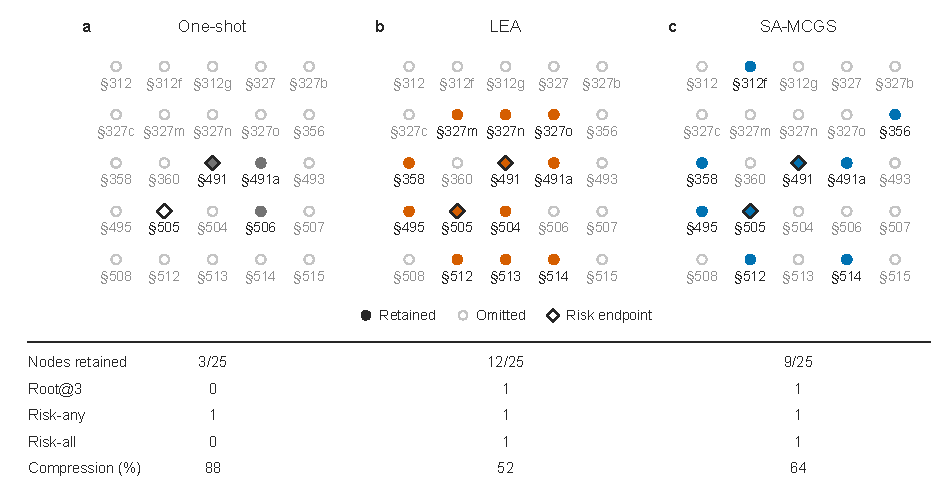
\includegraphics[width=\textwidth]{figures_restored_baseline/fig06_representative_scc_three_methods.pdf}
    \caption{Comparison of three methods on the same 25-record BGB case with Gemini 2.5 Pro. Node positions are fixed across panels; filled markers indicate retained records and open markers indicate omitted records. Diamonds mark the root (\S505) and witness (\S491). The rows below report retained node counts and the four evaluation metrics.}
    \label{fig:case}
\end{figure*}
